
  
\documentclass[journal,12pt,twocolumn]{IEEEtran}

\usepackage{setspace}
\usepackage{gensymb}
\singlespacing
\usepackage[cmex10]{amsmath}

\usepackage{amsthm}
\usepackage{commath}
\usepackage{mathrsfs}
\usepackage{txfonts}
\usepackage{stfloats}
\usepackage{bm}
\usepackage{cite}
\usepackage{cases}
\usepackage{subfig}

\usepackage{longtable}
\usepackage{multirow}

\usepackage{enumitem}
\usepackage{mathtools}
\usepackage{steinmetz}
\usepackage{tikz}
\usepackage{circuitikz}
\usepackage{verbatim}
\usepackage{tfrupee}
\usepackage[breaklinks=true]{hyperref}
\usepackage{graphicx}
\usepackage{tkz-euclide}

\usetikzlibrary{calc,math}
\usepackage{listings}
    \usepackage{color}                                            %%
    \usepackage{array}                                            %%
    \usepackage{longtable}                                        %%
    \usepackage{calc}                                             %%
    \usepackage{multirow}                                         %%
    \usepackage{hhline}                                           %%
    \usepackage{ifthen}                                           %%
    \usepackage{lscape}     
\usepackage{multicol}
\usepackage{chngcntr}

\DeclareMathOperator*{\Res}{Res}

\renewcommand\thesection{\arabic{section}}
\renewcommand\thesubsection{\thesection.\arabic{subsection}}
\renewcommand\thesubsubsection{\thesubsection.\arabic{subsubsection}}

\renewcommand\thesectiondis{\arabic{section}}
\renewcommand\thesubsectiondis{\thesectiondis.\arabic{subsection}}
\renewcommand\thesubsubsectiondis{\thesubsectiondis.\arabic{subsubsection}}


\hyphenation{op-tical net-works semi-conduc-tor}
\def\inputGnumericTable{}                                 %%

\lstset{
%language=C,
frame=single, 
breaklines=true,
columns=fullflexible
}
\begin{document}

\newcommand{\BEQA}{\begin{eqnarray}}
\newcommand{\EEQA}{\end{eqnarray}}
\newcommand{\define}{\stackrel{\triangle}{=}}
\bibliographystyle{IEEEtran}
\raggedbottom
\setlength{\parindent}{0pt}
\providecommand{\mbf}{\mathbf}
\providecommand{\pr}[1]{\ensuremath{\Pr\left(#1\right)}}
\providecommand{\qfunc}[1]{\ensuremath{Q\left(#1\right)}}
\providecommand{\sbrak}[1]{\ensuremath{{}\left[#1\right]}}
\providecommand{\lsbrak}[1]{\ensuremath{{}\left[#1\right.}}
\providecommand{\rsbrak}[1]{\ensuremath{{}\left.#1\right]}}
\providecommand{\brak}[1]{\ensuremath{\left(#1\right)}}
\providecommand{\lbrak}[1]{\ensuremath{\left(#1\right.}}
\providecommand{\rbrak}[1]{\ensuremath{\left.#1\right)}}
\providecommand{\cbrak}[1]{\ensuremath{\left\{#1\right\}}}
\providecommand{\lcbrak}[1]{\ensuremath{\left\{#1\right.}}
\providecommand{\rcbrak}[1]{\ensuremath{\left.#1\right\}}}
\theoremstyle{remark}
\newtheorem{rem}{Remark}
\newcommand{\sgn}{\mathop{\mathrm{sgn}}}
\providecommand{\abs}[1]{\vert#1\vert}
\providecommand{\res}[1]{\Res\displaylimits_{#1}} 
\providecommand{\norm}[1]{\lVert#1\rVert}
%\providecommand{\norm}[1]{\lVert#1\rVert}
\providecommand{\mtx}[1]{\mathbf{#1}}
\providecommand{\mean}[1]{E[ #1 ]}
\providecommand{\fourier}{\overset{\mathcal{F}}{ \rightleftharpoons}}
%\providecommand{\hilbert}{\overset{\mathcal{H}}{ \rightleftharpoons}}
\providecommand{\system}{\overset{\mathcal{H}}{ \longleftrightarrow}}
	%\newcommand{\solution}[2]{\textbf{Solution:}{#1}}
\newcommand{\solution}{\noindent \textbf{Solution: }}
\newcommand{\cosec}{\,\text{cosec}\,}
\providecommand{\dec}[2]{\ensuremath{\overset{#1}{\underset{#2}{\gtrless}}}}
\newcommand{\myvec}[1]{\ensuremath{\begin{pmatrix}#1\end{pmatrix}}}
\newcommand{\mydet}[1]{\ensuremath{\begin{vmatrix}#1\end{vmatrix}}}
\numberwithin{equation}{subsection}
\makeatletter
\@addtoreset{figure}{problem}
\makeatother
\let\StandardTheFigure\thefigure
\let\vec\mathbf
\renewcommand{\thefigure}{\theproblem}
\def\putbox#1#2#3{\makebox[0in][l]{\makebox[#1][l]{}\raisebox{\baselineskip}[0in][0in]{\raisebox{#2}[0in][0in]{#3}}}}
     \def\rightbox#1{\makebox[0in][r]{#1}}
     \def\centbox#1{\makebox[0in]{#1}}
     \def\topbox#1{\raisebox{-\baselineskip}[0in][0in]{#1}}
     \def\midbox#1{\raisebox{-0.5\baselineskip}[0in][0in]{#1}}
\vspace{3cm}
\title{Assignment 1}
\author{Adarsh Sai - AI20BTECH11001}
\maketitle
\newpage
\bigskip
\renewcommand{\thefigure}{\theenumi}
\renewcommand{\thetable}{\theenumi}
Download all python codes from 
\begin{lstlisting}
https://github.com/Adarsh541/EE3900/blob/main/EE3900_As1/codes/EE3900_As1.py
\end{lstlisting}

%
Download latex-tikz codes from 
%
\begin{lstlisting}
https://github.com/Adarsh541/EE3900/blob/main/EE3900_As1/EE3900_As1.tex
\end{lstlisting}
\section{Problem(Vectors Q2.1)}
The vertices of $\triangle$ABC are $\Vec{A}=\myvec{4\\6}$, $\Vec{B}=\myvec{1\\5}$ and $\Vec{C}=\myvec{7\\2}$. A line drawn to intersect sides AB and AC at D and E respectively, such that
\begin{align}
    \frac{AD}{AB}=\frac{AE}{AC}=\frac{1}{4}
\end{align}
Find 
\begin{align}
    \frac{\text{area of } \triangle ADE}{\text{area of } \triangle ABC}
\end{align}
\section{Solution}
\begin{align}
    \frac{AD}{AB}&=\frac{1}{4}\\
    \frac{AD}{AD+DB}&=\frac{1}{4}\\
    \implies \frac{AD}{DB}&=\frac{1}{3}
\end{align}
Similarly
\begin{align}
    \frac{AE}{EC}=\frac{1}{3}
\end{align}
$\vec{D}$ divides AB in the ratio $1:3$ internally. $\vec{E}$ divides AE in the ratio $1:3$ internally
\begin{align}
    \implies \vec{D} &=\frac{3\vec{A}+\vec{B}}{4}\\
    &=\myvec{\frac{13}{4}\\\\\frac{23}{4}}\\
    \vec{E} &=\frac{3\vec{A}+\vec{C}}{4}\\
    &=\myvec{\frac{19}{4}\\\\\frac{20}{4}}
\end{align}
\begin{align}
    \text{Area of } \triangle ABC &= \frac{1}{2}\norm{\brak{\vec{B-A}} \times \brak{\vec{C-A}}}\\
    &=\frac{1}{2}\norm{\myvec{-3\\-1}\times \myvec{3\\-4}}\\
    &=\frac{1}{2}\sbrak{\brak{-3\times -4}-\brak{-1 \times 3}}\\
    &=\frac{15}{2}
\end{align}
\begin{align}
    \text{Area of } \triangle ADE &= \frac{1}{2}\norm{\brak{\vec{D-A}} \times \brak{\vec{E-A}}}\\
    &=\frac{1}{2}\norm{\myvec{\frac{-3}{4}\\\\\frac{-1}{4}}\times \myvec{\frac{3}{4}\\\\\frac{-4}{4}}}\\
    &=\frac{1}{2}\sbrak{\brak{\frac{-3}{4}\times \frac{-4}{4}}-\brak{\frac{-1}{4} \times \frac{3}{4}}}\\
    &=\frac{15}{2\times16}
\end{align}
\begin{align}
    \frac{\text{area of } \triangle ADE}{\text{area of } \triangle ABC}=\frac{1}{16}
\end{align}
\begin{figure}[!h]
 \centering
 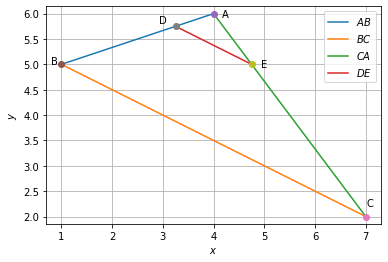
\includegraphics[width=\columnwidth]{figs.png}
 \caption{Plot of the triangles}
 \label{plot}
\end{figure}
\end{document}

